\documentclass[UTF8,AutoFakeBold,a4paper]{article}
\usepackage{ctex}
\usepackage{framed}
\usepackage{amsthm}
\usepackage{geometry}
\usepackage{amsthm,amsmath,amssymb}
\usepackage{mathrsfs}
\geometry{left=1cm,right=1cm,top=2.5cm,bottom=2.5cm}
\usepackage{amsmath}
\usepackage{graphicx}
\usepackage{multirow}
\usepackage{subfiles}
\linespread{1.314}
%\usepackage{luatexja-fontspec}
%\setCJKmainfont[ItalicFont=FandolKai-Regular,BoldFont=STSongti-SC-Black]{SimSun} 
\usepackage{physics}
\usepackage{graphicx}
%\setCJKfamilyfont{kaiti}{FandolKai-Regular}
%\newcommand{\kaiti}{\CJKfamily{kaiti}}%
\usepackage{paralist}
\everymath{\displaystyle}
\usepackage{chngcntr}%图片编号的宏包
\counterwithout{figure}{section}%取消图片按章节编号
%\counterwithin{figure}{section}%将equation环境重新编号,不按节编号
%\usepackage{emoji}
%\usepackage{ntheorem}
%\setemojifont{Twemoji Mozilla} 
%
%\usepackage{multicol}
%\let\itemize\compactitem
%\let\enditemize\endcompactitem
%\let\enumerate\compactenum
%\let\endenumerate\endcompactenum
%\let\description\compactdesc
%\let\enddescription\endcompactdesc
\usepackage{color}
\usepackage{fancyhdr} %调用宏包

% ---基本设置---

%设定页面的页眉页脚类型,$\LaTeX$内置了四种:empty、plain、headings及myheadings
\pagestyle{fancy}

%清除原页眉页脚样式
\fancyhf{} 

%R:页面右边;O:奇数页;\leftmark:表示“一级标题”
\fancyhead[CO]{\leftmark}

%L:页面左边;E:偶数页;\rightmark:表示“二级标题”
\fancyhead[CE]{\rightmark}

%C:页面中间
\fancyhead[CO, CE]{化工原理实验数据处理}

% 设置页脚,页眉的位置上也可以放置页码
\fancyfoot[CO]{\thepage}

% 设置页眉页脚横线及样式
%页眉线宽,设为0可以去页眉线
\renewcommand{\headrulewidth}{0.5pt} 

\usepackage{listings}

{
\lstset{numbers=left, %设置行号位置
        numberstyle=\zihao{-5}, %设置行号大小
        keywordstyle=\textcolor[rgb]{0.07,0.36,0.57}, %设置关键字颜色
        commentstyle=\textcolor[rgb]{0.21,0.49,0.30}, %设置注释颜色
        escapeinside=``, %逃逸字符(1左面的键),用于显示中文
        extendedchars=false, 
        xleftmargin=2em,xrightmargin=2em, aboveskip=1em, %设置边距
        tabsize=4, %设置tab空格数
        showspaces=false %不显示空格
       }

\title{\textbf{化工原理实验}}
\date{\today}
\author{B.H.Zhang}
%\setmainfont{Times New Roman}
%\setCJKsansfont{STSong}
%%\setCJKmainfont[BoldFont=STHeiti]{STSong}
%%\setCJKmainfont{STXihei}
%\setCJKmonofont{STXihei}
\usepackage{chemfig}
\usepackage{mathrsfs}
\usepackage{listings}
\usepackage{makeidx}
\makeindex
\usepackage{framed}
\usepackage{amsthm,amsmath,amssymb}
\usepackage{wrapfig}
\usepackage{graphicx}
\usepackage{mathrsfs}
\bibliographystyle{plain}
\usepackage{subfiles}
\usepackage{booktabs}
\usepackage{graphicx,times}
\usepackage{esint}
\usepackage{times}
\usepackage{subfigure}         
\usepackage{natbib}
\usepackage{amssymb,amsmath}
\usepackage{url}
\usepackage{geometry}
\usepackage{xcolor}
\usepackage{setspace}
\usepackage{subfigure}
\usepackage{booktabs}
\usepackage{array}
\usepackage{mhchem}
%\usepackage[usenames,dvipsnames]{color}
\usepackage{colortbl}
\usepackage{bm}
\usepackage{calligra}
\definecolor{mygray}{gray}{.9}
\definecolor{mypink}{rgb}{.99,.91,.95}
\definecolor{mycyan}{cmyk}{.3,0,0,0}
\definecolor{myorgn}{rgb}{0.56,0.28,0.16}
\definecolor{myyelo}{rgb}{255,215,0}
\usepackage{environ}
\everymath{\displaystyle}  
\usepackage[breaklinks,colorlinks,linkcolor=black,citecolor=black,urlcolor=black]{hyperref}
\usepackage{tikz}
\begin{document}
\maketitle
\section{流体阻力测定}


\begin{table}[h]
		\centering
		\begin{tabular}{cccccccc}
		\toprule
		
 序号 & 流量$Q$ & 压差$\Delta p$ & 水温$\theta$ & 水的密度$\rho$ & 水的粘度$\mu$ & 直管摩擦系数$\lambda$ & 雷诺数$Re$ \\ 
  (量纲)&$\rm{L}\cdot\rm{h}^{-1}$&Pa&$^{\circ}$C&kg$\cdot\rm{m}^{-3}$&Pa$\cdot$s&1&1\\
 \midrule
		1 & 10 & 98.10 & 20.40 & 998.1225 & 0.00099236 & 0.2881 & 456.07 \\ 
        2 & 14 & 137.34 & 20.50 & 998.1013 & 0.00098995 & 0.2058 & 640.03 \\ 
        3 & 20 & 147.15 & 20.50 & 998.1013 & 0.00098995 & 0.1080 & 914.33 \\ 
        4 & 30 & 206.01 & 20.60 & 998.0801 & 0.00098754 & 0.0672 & 1374.82 \\ 
        5 & 40 & 343.35 & 20.60 & 998.0801 & 0.00098754 & 0.0630 & 1833.09 \\ 
        \rowcolor{mypink}
        6 & 50 & 519.93 & 20.70 & 998.0590 & 0.00098513 & 0.0611 & 2296.92 \\ 
        \rowcolor{mypink}
        7 & 60 & 618.03 & 20.70 & 998.0590 & 0.00098513 & 0.0504 & 2756.30 \\ 
        \rowcolor{mypink}
        8 & 80 & 990.81 & 20.70 & 998.0590 & 0.00098513 & 0.0455 & 3675.07 \\ 
        9 & 100 & 1530.36 & 20.80 & 998.0378 & 0.00098272 & 0.0449 & 4605.01 \\ 
        10 & 160 & 2766.42 & 20.80 & 998.0378 & 0.00098272 & 0.0317 & 7368.01 \\ 
        11 & 200 & 4071.15 & 20.80 & 998.0378 & 0.00098272 & 0.0299 & 9210.01 \\ 
        12 & 280 & 8260.02 & 20.90 & 998.0167 & 0.00098031 & 0.0309 & 12925.44 \\ 
        13 & 360 & 11600.00 & 20.90 & 998.0167 & 0.00098031 & 0.0263 & 16618.43 \\ 
        14 & 400 & 14200.00 & 20.90 & 998.0167 & 0.00098031 & 0.0261 & 18464.92 \\ 
        15 & 600 & 28700.00 & 20.90 & 998.0167 & 0.00098031 & 0.0234 & 27697.38 \\ 
        16 & 800 & 48600.00 & 20.90 & 998.0167 & 0.00098031 & 0.0223 & 36929.83 \\ 
        17 & 1200 & 101200.00 & 21.00 & 997.9955 & 0.00097790 & 0.0206 & 55530.09 \\ 
        18 & 1600 & 166800.00 & 21.00 & 997.9955 & 0.00097790 & 0.0191 & 74040.12 \\ 
        \bottomrule
		\end{tabular}	
		\label{ta1}
		\caption{流体阻力数据计算整理,过度区在表中用\textcolor{mypink}{粉色}标出了}
\end{table}

\begin{table}[h]
		\centering
		\begin{tabular}{cccccc}
		\toprule
		
 序号 & 近端压差 & 远端压差 & 流体温度 & 局部阻力引起的能量损失 & 局部阻力系数 \\ 
  (量纲)&Pa&Pa&$^{\circ}$C&J$\cdot$kg&1\\
 \midrule
		1 & 76500.00 & 78200.00 & 21.35 & 74.93 & 15.16 \\ 
        2 & 61600.00 & 62800.00 & 21.60 & 60.51 & 15.12 \\ 
        3 & 48200.00 & 50800.00 & 21.80 & 45.69 & 14.45 \\ 
        4 & 37600.00 & 38700.00 & 22.05 & 36.57 & 15.10 \\ 
        5 & 28300.00 & 29100.00 & 22.25 & 27.56 & 15.49 \\ 
        \bottomrule
		\end{tabular}	
		\label{ta1}
		\caption{局部阻力实验数据处理}
\end{table}



\newpage


\begin{figure}[h]
	\centering
	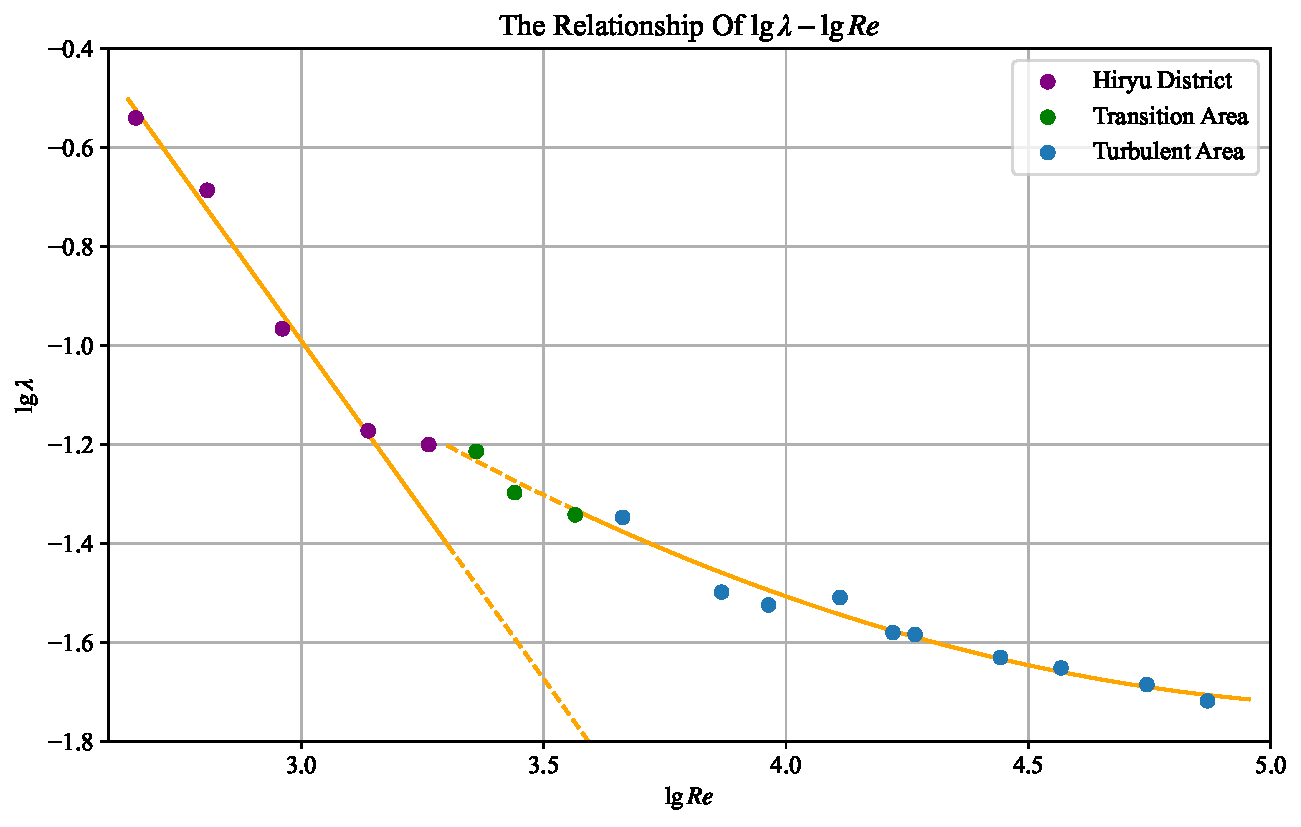
\includegraphics[scale=0.5]{流体阻力1}
	\caption{直管摩擦系数$\lambda$与雷诺数$Re$之间的关系(采用双对数坐标),其中层流、过度、湍流用不同颜色的点进行标出。并在过度区域使用虚线进行分隔。}
\end{figure}


\newpage

\setlength{\tabcolsep}{1mm}{
\begin{table}[h]
		\centering
		\begin{tabular}{cccccccccc}
		\toprule
		压力差$\Delta p$ & 流量$Qe$ & 功率 & 水温$t$ & 水的密度$\rho$ & 压头$H$ & 扬程$He$ & 有效功率$Ne$ & 轴功率$N$ & 效率$\eta$\\ 
		Pa&$\rm{m}^{3}\cdot\rm{s}^{-1}$&kW&$^{\circ}\rm{C}$&$\rm{kg}\cdot\rm{m}^{-3}$&m&m&kW&kW&100\%\\
		\midrule
        220000 & 0.0000000 & 0.32 & 20.8 & 998.03366 & 22.49 & 22.67 & 0.0000 & 0.192 & 0.00 \\ 
        195000 & 0.0006930 & 0.44 & 20.9 & 998.01198 & 19.94 & 20.12 & 0.1364 & 0.264 & 51.67 \\ 
        185000 & 0.0009773 & 0.49 & 20.9 & 998.01198 & 18.92 & 19.10 & 0.1826 & 0.294 & 62.10 \\ 
        175000 & 0.0011949 & 0.53 & 21.0 & 997.99030 & 17.89 & 18.07 & 0.2113 & 0.318 & 66.44 \\ 
        169000 & 0.0013780 & 0.57 & 21.0 & 997.99030 & 17.28 & 17.46 & 0.2354 & 0.342 & 68.83 \\ 
        163000 & 0.0015392 & 0.59 & 21.1 & 997.96862 & 16.67 & 16.85 & 0.2537 & 0.354 & 71.67 \\ 
        157000 & 0.0016849 & 0.61 & 21.2 & 997.94694 & 16.05 & 16.23 & 0.2676 & 0.366 & 73.11 \\ 
        151000 & 0.0018187 & 0.62 & 21.3 & 997.92526 & 15.44 & 15.62 & 0.2779 & 0.372 & 74.71 \\ 
        145000 & 0.0019432 & 0.64 & 21.4 & 997.90358 & 14.83 & 15.01 & 0.2853 & 0.384 & 74.30 \\ 
        139000 & 0.0020600 & 0.65 & 21.5 & 997.88190 & 14.21 & 14.39 & 0.2901 & 0.39 & 74.38 \\ 
        131000 & 0.0021705 & 0.66 & 21.6 & 997.86022 & 13.40 & 13.58 & 0.2883 & 0.396 & 72.80 \\ 
        125000 & 0.0022755 & 0.67 & 21.6 & 997.86022 & 12.78 & 12.96 & 0.2886 & 0.402 & 71.78 \\ 
        119000 & 0.0023758 & 0.67 & 21.7 & 997.83854 & 12.17 & 12.35 & 0.2870 & 0.402 & 71.40 \\ 
        113000 & 0.0024642 & 0.67 & 21.8 & 997.81686 & 11.56 & 11.74 & 0.2829 & 0.402 & 70.37 \\ 
        110000 & 0.0025187 & 0.67 & 21.8 & 997.81686 & 11.25 & 11.43 & 0.2816 & 0.402 & 70.05 \\ \bottomrule
		\end{tabular}	
		\label{ta1}
		\caption{离心泵实验数据计算整理}
\end{table}}

\begin{table}[h]
		\centering
		\begin{tabular}{ccccccc}
		\toprule
		编号 & 压力差$\Delta p$ & 流量$Qe$ & 水温$t$ & 水的密度$\rho$ & 压头$H$ & 扬程$He$\\ 
		&Pa&$\rm{m}^{3}\cdot\rm{s}^{-1}$&$^{\circ}\rm{C}$&$\rm{kg}\cdot\rm{m}^{-3}$&m&m\\
		\midrule
        15 & 7000 & 0.0003485 & 22.4 & 997.6777 & 0.716 & 0.8959 \\ 
        14 & 10000 & 0.0004915 & 22.4 & 997.6777 & 1.023 & 1.2028 \\ 
        13 & 12000 & 0.0006930 & 22.3 & 997.7004 & 1.227 & 1.4073 \\ 
        12 & 15000 & 0.0008474 & 22.3 & 997.7004 & 1.534 & 1.7141 \\ 
        11 & 18000 & 0.0010168 & 22.3 & 997.7004 & 1.841 & 2.0210 \\ 
        10 & 22000 & 0.0011949 & 22.3 & 997.7004 & 2.250 & 2.4301 \\ 
        9 & 31000 & 0.0013493 & 22.3 & 997.7004 & 3.171 & 3.3506 \\ 
        8 & 40000 & 0.0015136 & 22.3 & 997.7004 & 4.091 & 4.2710 \\ 
        7 & 49000 & 0.0016732 & 22.3 & 997.7004 & 5.012 & 5.1915 \\ 
        6 & 58000 & 0.0018294 & 22.3 & 997.7004 & 5.932 & 6.1120 \\ 
        5 & 67000 & 0.0019829 & 22.2 & 997.7231 & 6.852 & 7.0323 \\ 
        4 & 78000 & 0.0021343 & 22.2 & 997.7231 & 7.977 & 8.1573 \\ 
        3 & 87000 & 0.0022670 & 22.1 & 997.7458 & 8.898 & 9.0776 \\ 
        2 & 101000 & 0.0024003 & 22.0 & 997.7685 & 10.329 & 10.5092 \\ 
        1 & 110000 & 0.0024955 & 21.9 & 997.7912 & 11.249 & 11.4293\\
        \bottomrule
		\end{tabular}	
		\label{ta1}
		\caption{管路实验数据计算整理}
\end{table}
\newpage
\section{流体输送综合实验}
\begin{figure}[h]
	\centering
	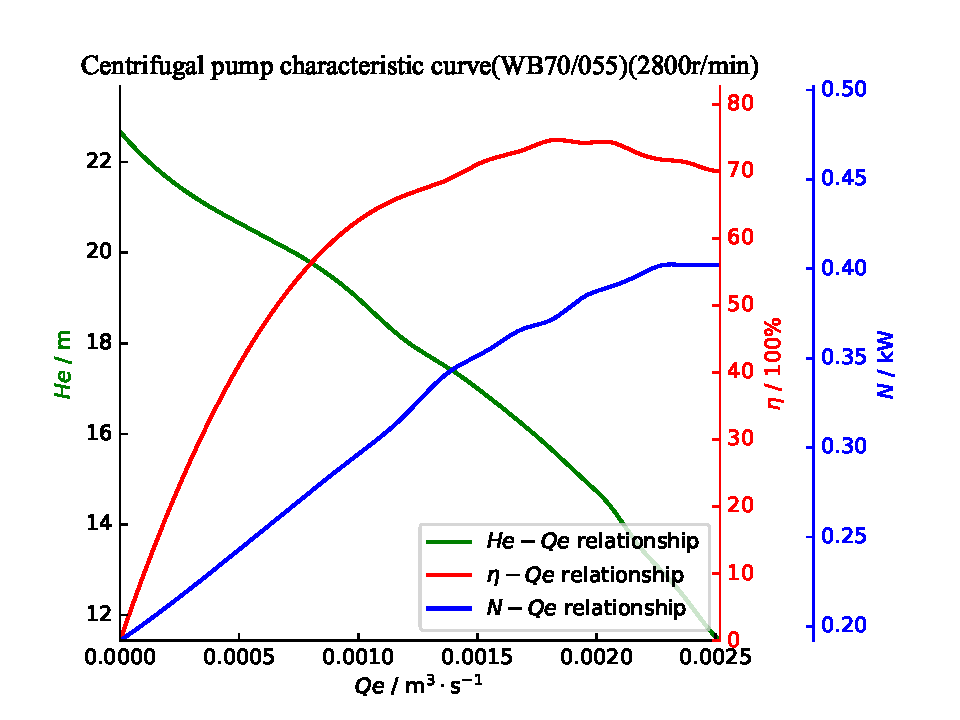
\includegraphics[scale=0.6]{离心泵特性曲线}
	\caption{离心泵的特性曲线,其泵型号为WB70/055,转速为2800r/min。该图有三根坐标轴,三条曲线,均在坐标轴旁做了标记。}
	
	\centering
	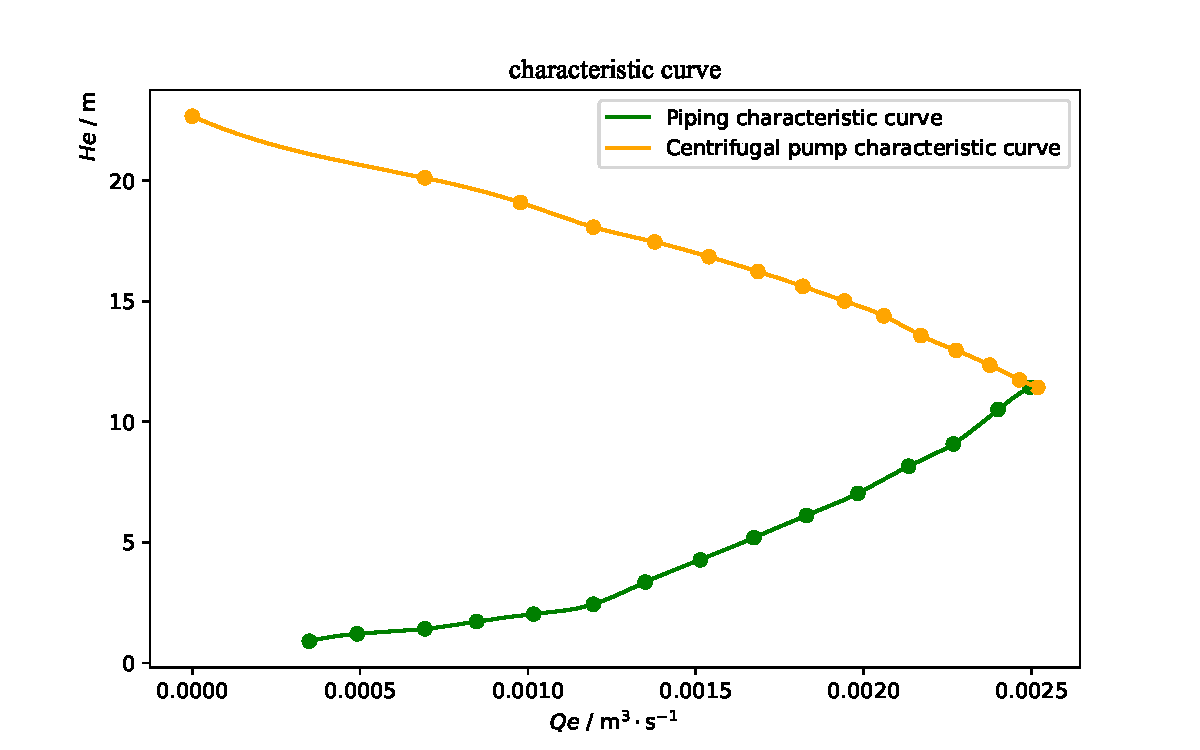
\includegraphics[scale=0.6]{管路特性曲线}
	\caption{管路的特性曲线、离心泵的特性曲线,其交点即为工作点。横坐标为流量(去单位$\rm{m}^{3}/\rm{s}$),纵坐标为扬程(去单位$\rm{m}$)。}
	
\end{figure}







\newpage
	\section{流量计标定及流量系数测定}
\begin{figure}[h]
	\centering
	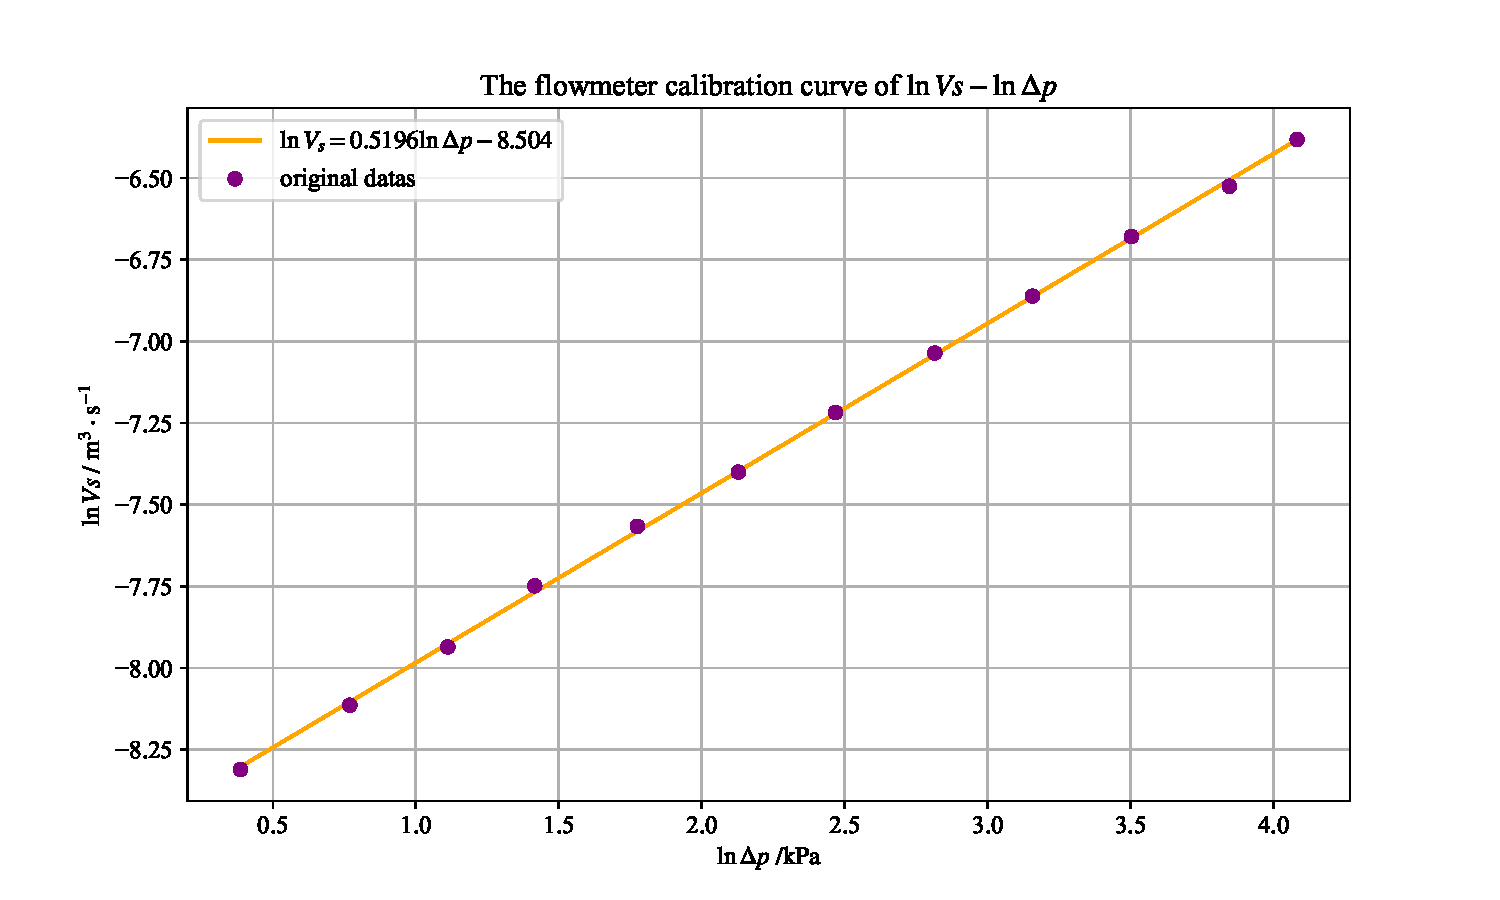
\includegraphics[scale=0.5]{文丘里1}
	\caption{节流式流量计(这里使用的流量计是文丘里流量计)的流量标定曲线(双对数坐标):纵坐标为节流式流量计的流量$V_{s}$(去单位为$\rm{m}^{3}\cdot\rm{s}^{-1}$),纵坐标为压差$\Delta p$(去单位为kPa)。}
	\label{fi1}
	
	\centering
	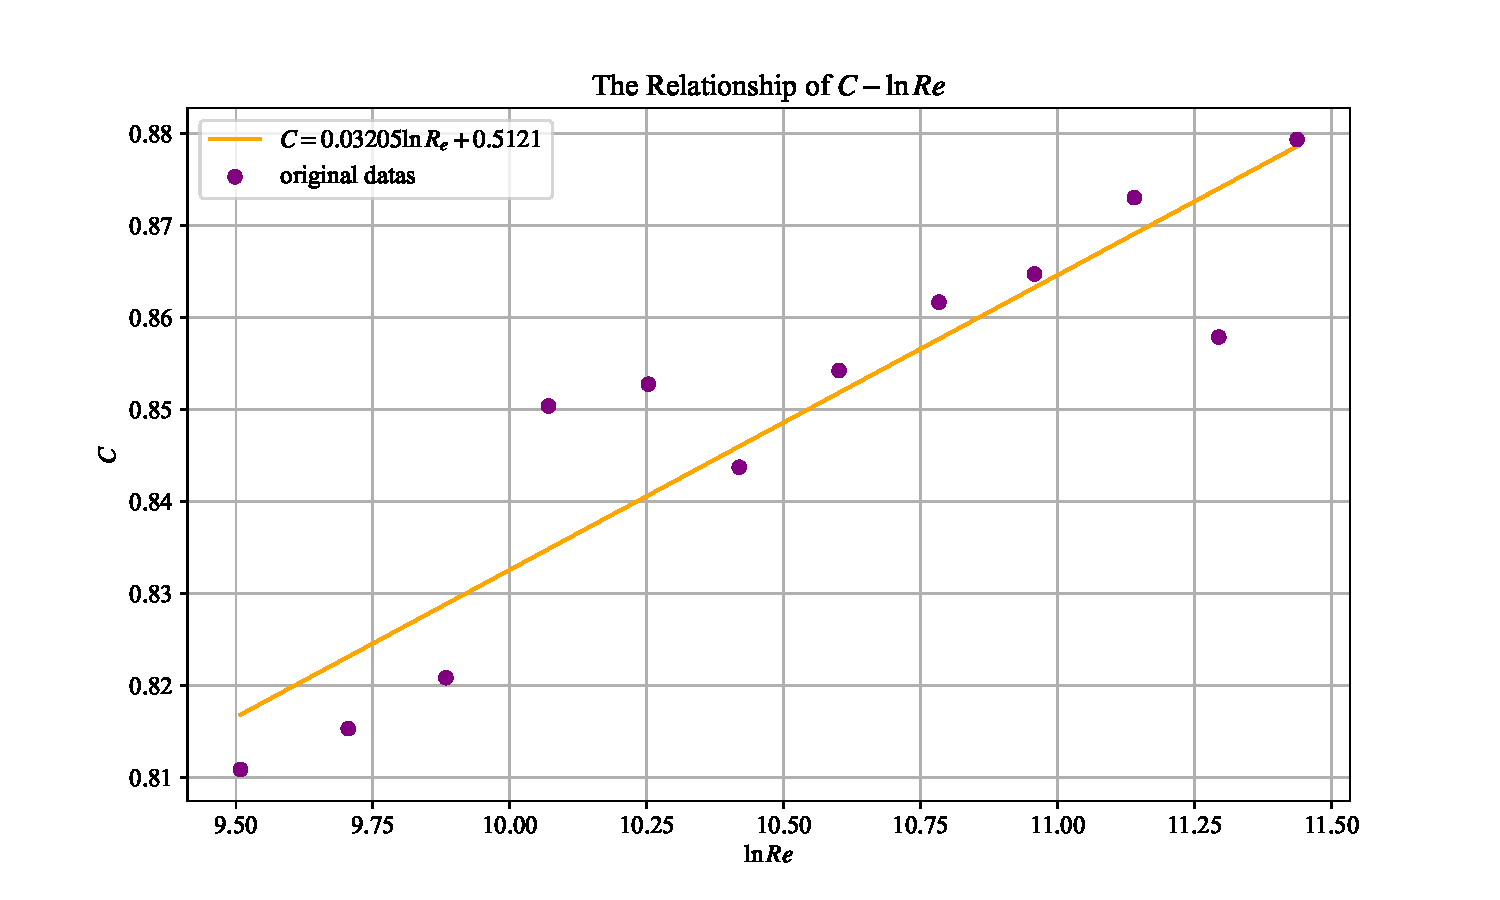
\includegraphics[scale=0.5]{文丘里2.pdf}
	\caption{流量系数$C$与雷诺准数$R_{e}$的关系曲线(单对数坐标)}
	\label{fi2}
\end{figure}

\newpage
\begin{figure}[h]
	\centering
	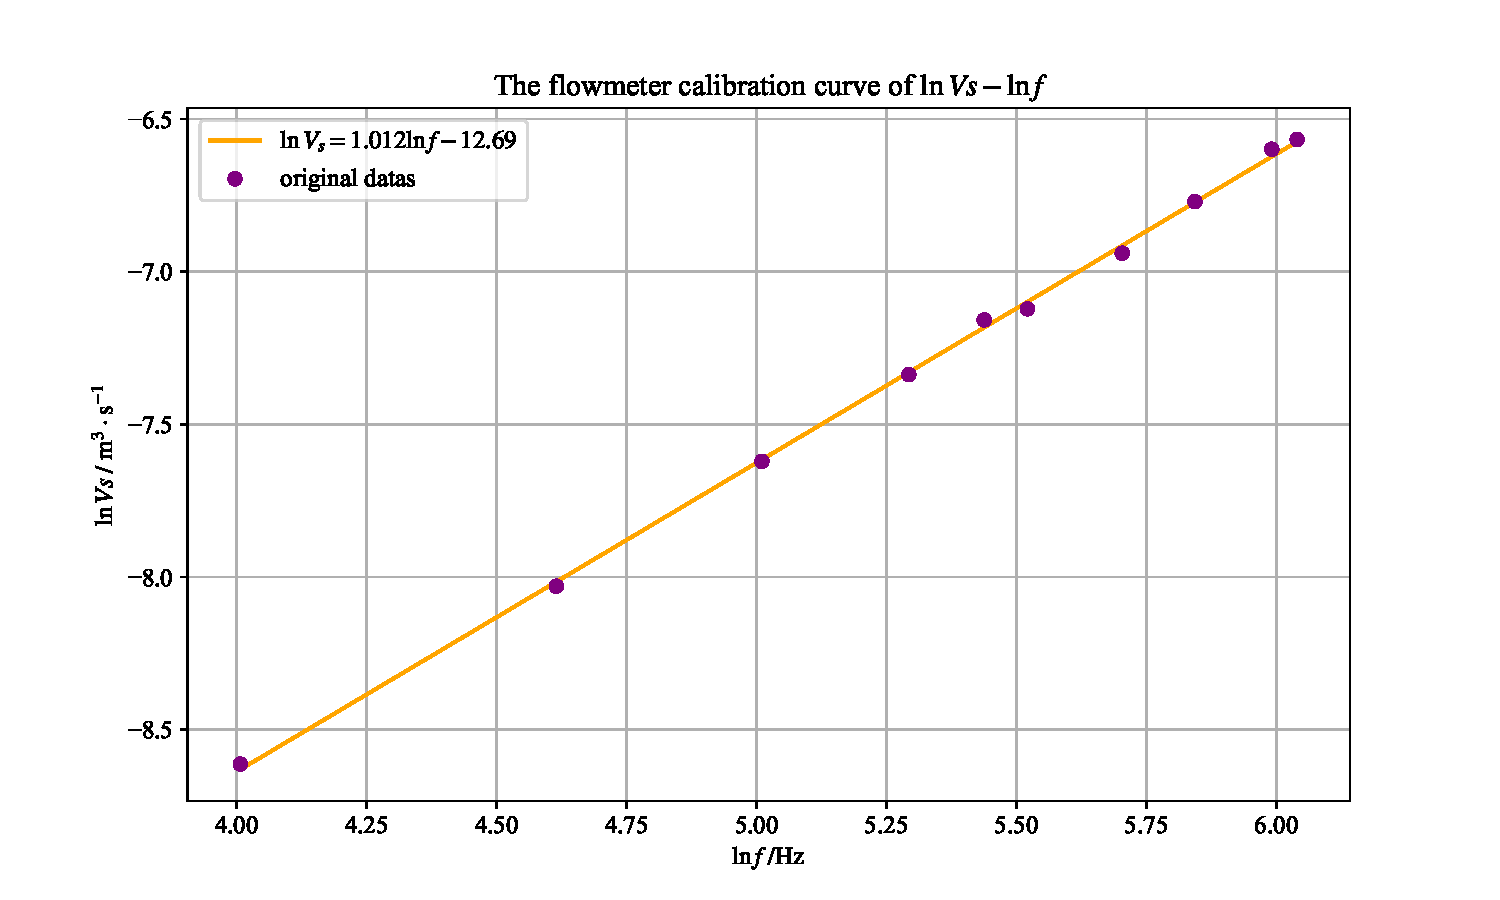
\includegraphics[scale=0.5]{涡轮1}
	\caption{涡轮流量计的流量标定曲线(双对数坐标):纵坐标为涡轮流量计的流量$V_{s}$(去单位为$\rm{m}^{3}\cdot\rm{s}^{-1}$),纵坐标为频率$f$(去单位为Hz)。}
	\label{fi3}
	
	\centering
	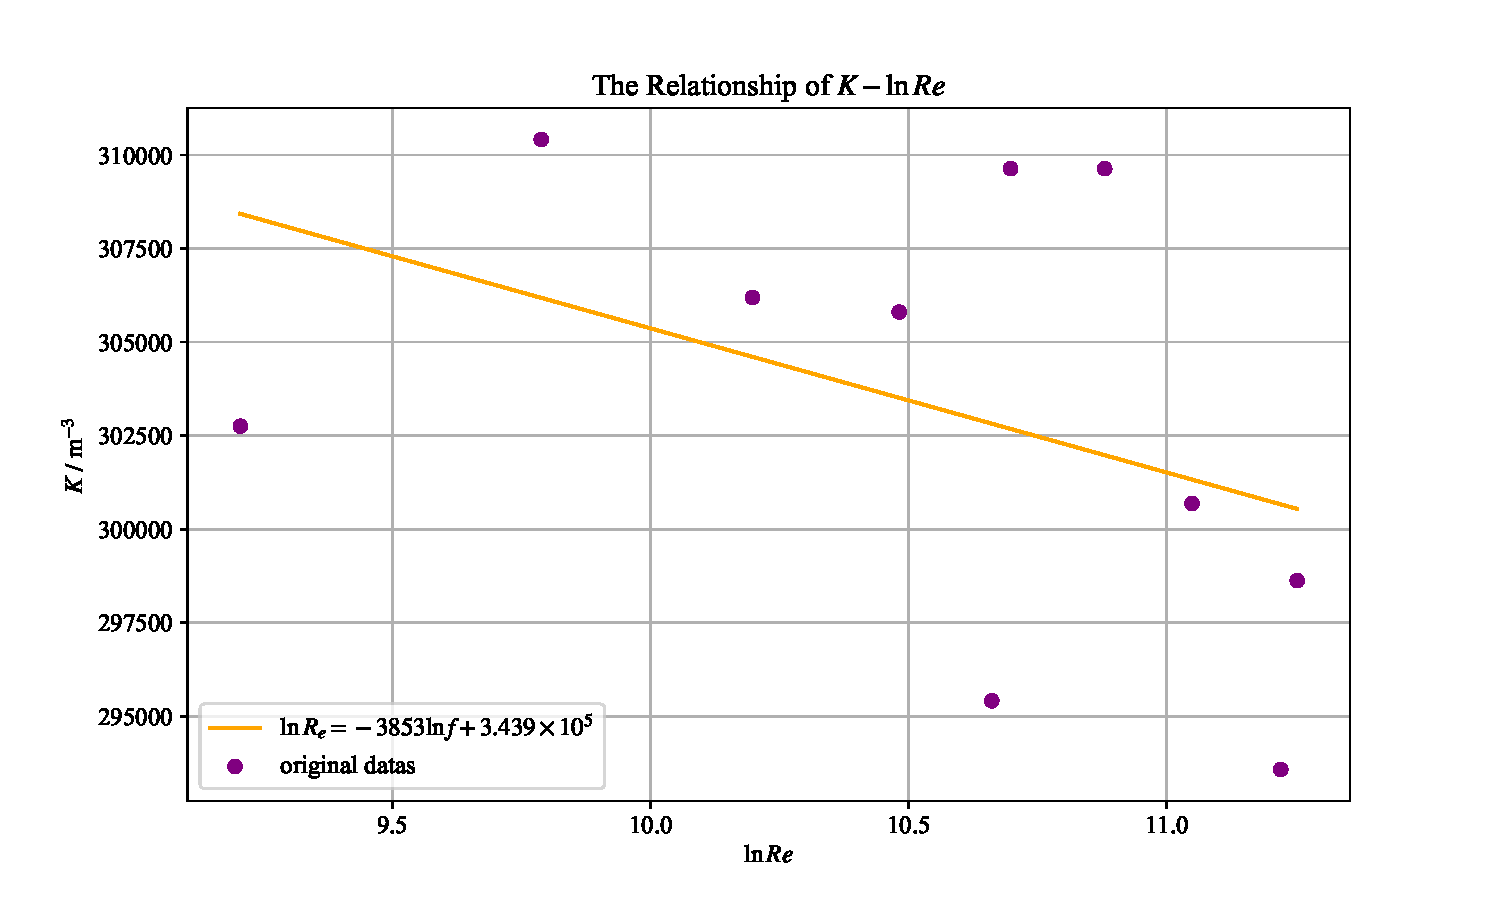
\includegraphics[scale=0.5]{涡轮2}
	\caption{仪表常数$K$(去单位为m$^{-3}$)与雷诺准数$R_{e}$的关系曲线(单对数坐标)}
	\label{fi4}
\end{figure}



\newpage
\begin{figure}[h]
	\centering
	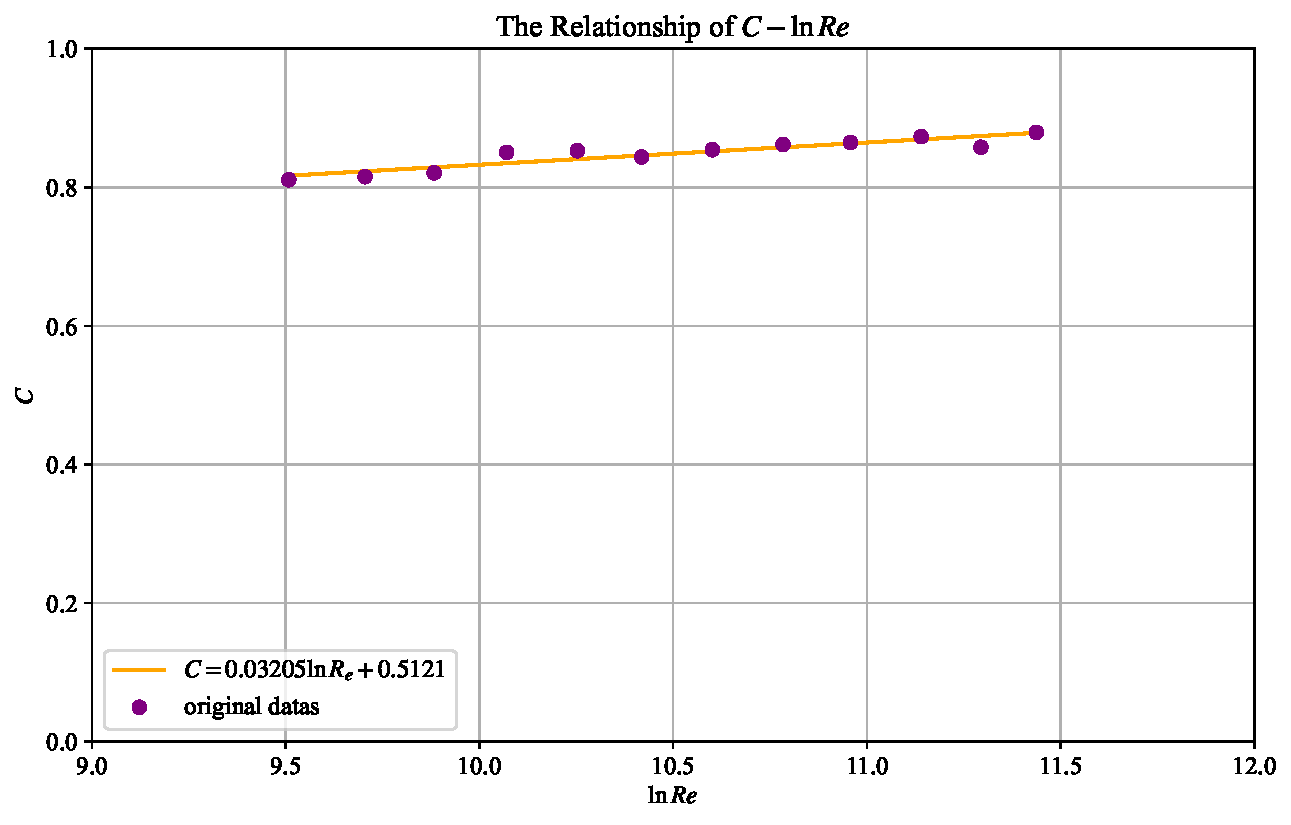
\includegraphics[scale=0.5]{文丘里3}
	\caption{流量系数$C$与雷诺准数$R_{e}$的关系曲线(单对数坐标从0开始)}
	\label{fi3}
	
	\centering
	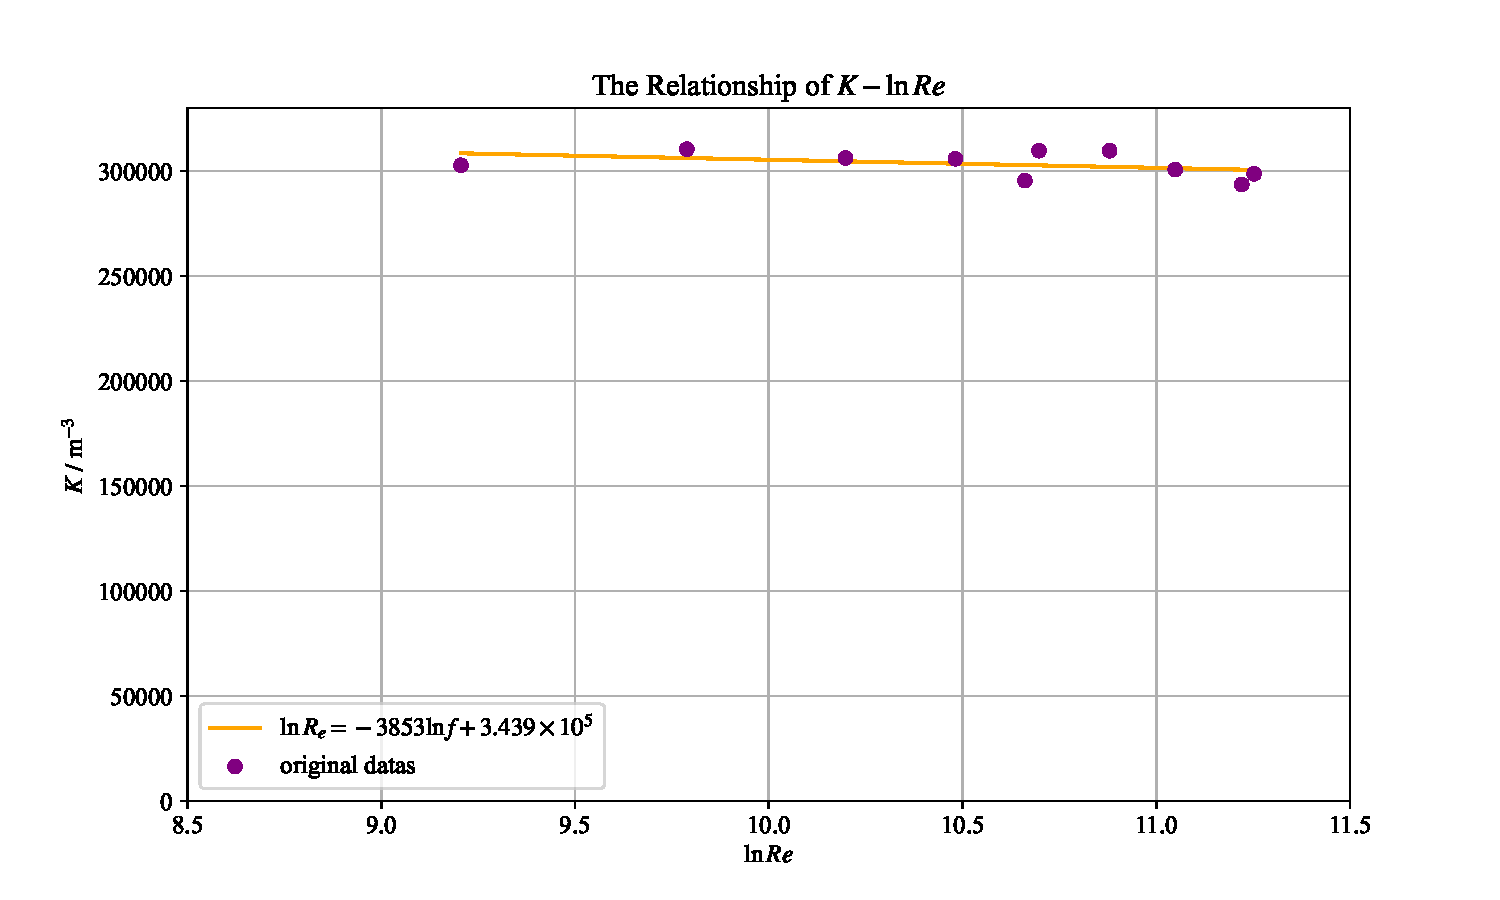
\includegraphics[scale=0.5]{涡轮3}
	\caption{仪表常数$K$(去单位为m$^{-3}$)与雷诺准数$R_{e}$的关系曲线(单对数坐标从0开始)}
	\label{fi4}
\end{figure}



\newpage

\begin{table}[h]
		\centering
		\begin{tabular}{cccccccc}
		\toprule
		
 序号 & 压差 & 液面高度差 & 平均用时 & 体积流量 & 流速 & 雷诺数 & 流量计系数 \\ 
  &$\Delta p/\rm{kPa}$&$\Delta h$&$\Delta t$&$V_{s}/\rm{m}^{3}\cdot\rm{s}^{-1}$&$u/\rm{m}\cdot\rm{s}^{-1}$&$R_{e}$&$C$\\
 \midrule
		1 & 1.471 & 200.0 & 89.50 & 0.0002458 & 0.4630 & 13469 & 0.8108 \\ 
        2 & 2.158 & 200.0 & 73.50 & 0.0002993 & 0.5638 & 16401 & 0.8153 \\ 
        3 & 3.041 & 200.0 & 61.50 & 0.0003577 & 0.6738 & 19602 & 0.8208 \\ 
        4 & 4.120 & 200.0 & 51.00 & 0.0004314 & 0.8125 & 23637 & 0.8504 \\ 
        5 & 5.900 & 200.0 & 42.50 & 0.0005176 & 0.9750 & 28365 & 0.8527 \\ 
        6 & 8.400 & 200.0 & 36.00 & 0.0006111 & 1.151 & 33486 & 0.8437 \\ 
        7 & 11.80 & 200.0 & 30.00 & 0.0007333 & 1.381 & 40183 & 0.8542 \\ 
        8 & 16.70 & 200.0 & 25.00 & 0.0008800 & 1.657 & 48220 & 0.8617 \\ 
        9 & 23.50 & 200.0 & 21.00 & 0.001048 & 1.973 & 57405 & 0.8647 \\ 
        10 & 33.20 & 200.0 & 17.50 & 0.001257 & 2.368 & 68886 & 0.8730 \\ 
        11 & 46.80 & 200.0 & 15.00 & 0.001467 & 2.762 & 80367 & 0.8579 \\ 
        12 & 59.30 & 200.0 & 13.00 & 0.001692 & 3.187 & 92731 & 0.8794 \\ 
		\bottomrule
		\end{tabular}	
		\label{ta1}
		\caption{文丘里流量计实验数据处理(计算示例见上)}
\end{table}


\begin{table}[h]
		\centering
		\begin{tabular}{cccccccc}
		\toprule
		
 序号 & 频率计读数 & 液面高度差 & 平均用时 & 体积流量 & 流速 & 雷诺数 & 仪表常数 \\ 
 &$f$&$\Delta h$&$\Delta t$&$V_{s}/\rm{m}^{3}\cdot\rm{s}^{-1}$&$u/\rm{m}\cdot\rm{s}^{-1}$&$R_{e}$&$K/\rm{m}^{-3}$\\
 \midrule
        1 & 55 & 200.0 & 120.0 & 0.0001817 & 0.3420 & 9955 & 302752 \\ 
        2 & 101 & 200.0 & 67.0 & 0.0003254 & 0.6130 & 17829 & 310413 \\ 
        3 & 150 & 200.0 & 44.5 & 0.0004899 & 0.9230 & 26844 & 306193 \\ 
        4 & 199 & 200.0 & 33.5 & 0.0006507 & 1.230 & 35658 & 305803 \\ 
        5 & 250 & 200.0 & 27.0 & 0.0008074 & 1.520 & 44242 & 309633 \\ 
        6 & 300 & 200.0 & 22.5 & 0.0009689 & 1.820 & 53091 & 309633 \\ 
        7 & 345 & 200.0 & 19.0 & 0.001147 & 2.160 & 62871 & 300688 \\ 
        8 & 400 & 200.0 & 16.0 & 0.001362 & 2.570 & 74659 & 293578 \\ 
        9 & 420 & 200.0 & 15.5 & 0.001406 & 2.650 & 77067 & 298624 \\ 
        10 & 230 & 200.0 & 28.0 & 0.0007786 & 1.470 & 42662 & 295413 \\ 
		\bottomrule
		\end{tabular}	
		\label{ta1}
		\caption{涡轮流量计实验数据处理(计算示例见上)}
\end{table}


\newpage

\section{传热综合}
\setlength{\tabcolsep}{0.4mm}{
\begin{table}[h]
		\centering
		\begin{tabular}{cccccccccccccc}
		\toprule
		
  序号 & 流量计读数 & ${t_{1}}_{i}$ & ${t_{m}}_{i}$ & 压降 & $\rho_{i}$ & $\mu_{i}$ & $\lambda_{i}$ & $C_{p}$ & $V_{i}$ & $\alpha$ & $Nu$ & $Re$ & $Pr$ \\
 量纲&kPa&$^\circ$C&$^\circ$C&kPa&$\rm{kg}\cdot\rm{m}^{-3}$&$\rm{kg}/m\cdot s$&W/m$\cdot$K&J/K&m$^{3}/\rm{h}$&W/m$\cdot$$^\circ$C&1&1&1\\
 \midrule
         1 & 0.21 & 39.40 & 38.14 & 0.25 & 1.1337 & 0.00001909 & 0.02648 & 1007 & 0.003219 & 50.32 & 36.57 & 11151 & 0.7261 \\ 
        2 & 0.29 & 39.50 & 38.35 & 0.31 & 1.1329 & 0.00001910 & 0.02650 & 1007 & 0.003782 & 58.30 & 42.36 & 13096 & 0.7260 \\ 
        3 & 0.39 & 40.00 & 38.19 & 0.40 & 1.1335 & 0.00001910 & 0.02649 & 1007 & 0.004383 & 66.50 & 48.33 & 15180 & 0.7261 \\ 
        4 & 0.53 & 40.40 & 38.36 & 0.50 & 1.1329 & 0.00001910 & 0.02650 & 1007 & 0.005106 & 75.59 & 54.91 & 17678 & 0.7260 \\ 
        5 & 0.73 & 40.90 & 38.20 & 0.66 & 1.1335 & 0.00001910 & 0.02649 & 1007 & 0.005988 & 87.18 & 63.36 & 20738 & 0.7261 \\ 
        6 & 1.00 & 41.50 & 37.97 & 0.86 & 1.1343 & 0.00001909 & 0.02647 & 1007 & 0.007001 & 100.72 & 73.25 & 24263 & 0.7261 \\ 
        7 & 1.37 & 42.20 & 37.70 & 1.12 & 1.1353 & 0.00001907 & 0.02645 & 1007 & 0.008186 & 116.06 & 84.47 & 28386 & 0.7262 \\ 
        8 & 1.88 & 43.00 & 37.35 & 1.49 & 1.1365 & 0.00001906 & 0.02642 & 1007 & 0.009577 & 133.20 & 97.04 & 33238 & 0.7263 \\ 
        9 & 2.58 & 44.20 & 36.93 & 1.98 & 1.1381 & 0.00001904 & 0.02639 & 1007 & 0.011198 & 151.99 & 110.86 & 38904 & 0.7264 \\ 
        10 & 3.45 & 45.50 & 36.25 & 2.58 & 1.1405 & 0.00001901 & 0.02634 & 1007 & 0.012923 & 171.56 & 125.37 & 44970 & 0.7266 \\ 		\bottomrule
		\end{tabular}	
		\label{ta1}
		\caption{普通管数据及其处理}
\end{table}}

\setlength{\tabcolsep}{0.4mm}{
\begin{table}[h]
		\centering
		\begin{tabular}{ccccccccccccccc}
		\toprule
		
  序号 & 流量计读数 & ${t_{1}}_{i}$ & ${t_{m}}_{i}$ & 压降 & $\rho_{i}$ & $\mu_{i}$ & $\lambda_{i}$ & $C_{p}$ & $V_{i}$ & $\alpha$ & $Nu$ & $Re$ & $Pr$ &$\dfrac{Nu}{Nu_{0}}$ \\
  量纲&kPa&$^\circ$C&$^\circ$C&kPa&$\rm{kg}\cdot\rm{m}^{-3}$&$\rm{kg}/m\cdot s$&W/m$\cdot$K&J/K&m$^{3}/\rm{h}$&W/m$\cdot$$^\circ$C&1&1&1&1\\
 \midrule
       1 & 0.21 & 41.30 & 36.94 & 0.25 & 1.1380 & 0.00001904 & 0.02639 & 1007 & 0.003209 & 50.48 & 36.82 & 11149 & 0.7264 & 1.007 \\ 
        2 & 0.28 & 41.00 & 36.98 & 0.32 & 1.1379 & 0.00001904 & 0.02640 & 1007 & 0.003708 & 58.92 & 42.97 & 12879 & 0.7264 & 1.015 \\ 
        3 & 0.37 & 40.90 & 36.77 & 0.43 & 1.1386 & 0.00001903 & 0.02638 & 1007 & 0.004263 & 68.72 & 50.14 & 14814 & 0.7265 & 1.038 \\ 
        4 & 0.50 & 41.00 & 36.56 & 0.57 & 1.1394 & 0.00001902 & 0.02637 & 1007 & 0.004954 & 81.01 & 59.15 & 17227 & 0.7265 & 1.077 \\ 
        5 & 0.67 & 41.20 & 36.23 & 0.75 & 1.1406 & 0.00001901 & 0.02634 & 1007 & 0.005733 & 94.58 & 69.12 & 19951 & 0.7266 & 1.091 \\ 
        6 & 0.91 & 41.50 & 35.98 & 1.02 & 1.1415 & 0.00001900 & 0.02632 & 1007 & 0.006678 & 110.65 & 80.92 & 23254 & 0.7267 & 1.105 \\ 
        7 & 1.22 & 42.00 & 35.87 & 1.34 & 1.1419 & 0.00001899 & 0.02631 & 1007 & 0.007726 & 126.26 & 92.37 & 26911 & 0.7267 & 1.094 \\ 
        8 & 1.64 & 42.60 & 35.36 & 1.77 & 1.1437 & 0.00001897 & 0.02628 & 1007 & 0.008949 & 147.50 & 108.06 & 31209 & 0.7269 & 1.114 \\ 
        9 & 2.22 & 43.30 & 35.03 & 2.32 & 1.1449 & 0.00001895 & 0.02625 & 1007 & 0.010400 & 170.07 & 124.71 & 36299 & 0.7269 & 1.125 \\ 
        10 & 3.00 & 44.50 & 34.26 & 3.11 & 1.1477 & 0.00001892 & 0.02620 & 1007 & 0.012067 & 196.46 & 144.37 & 42194 & 0.7272 & 1.152 \\ 
		\bottomrule
		\end{tabular}	
		\label{ta1}
		\caption{强化管数据及其处理}
\end{table}}
\newpage
\begin{figure}[h]
	\centering
	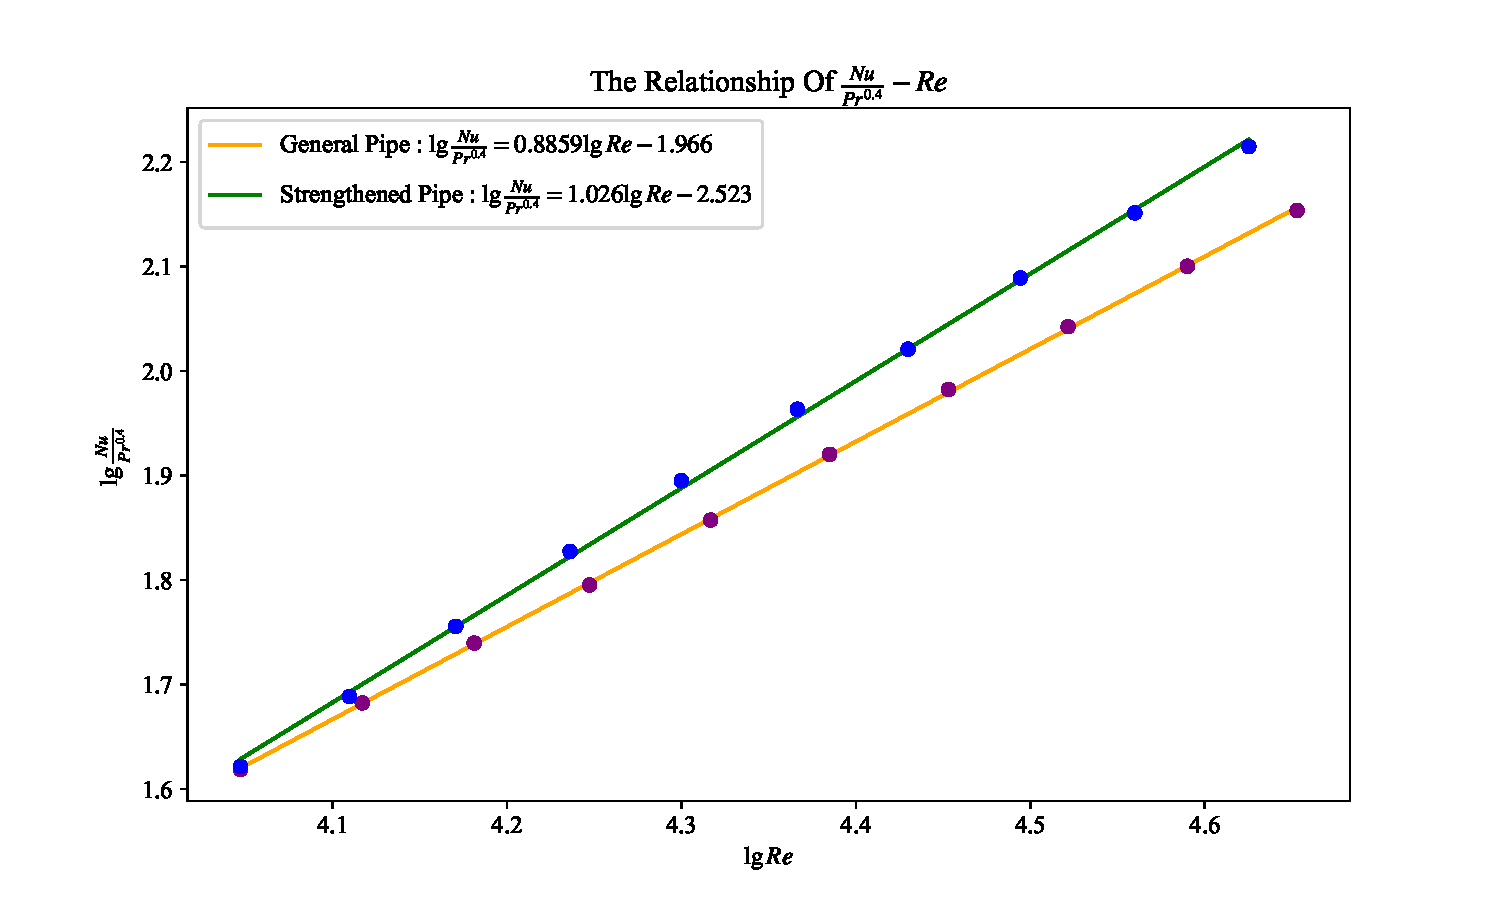
\includegraphics[scale=0.5]{强化普通}
	\caption{强化管、普通管的$\frac{Nu}{Pr^{0.4}}$与$Re$之关系(双对数坐标)}
	\label{fi3}
	\centering
	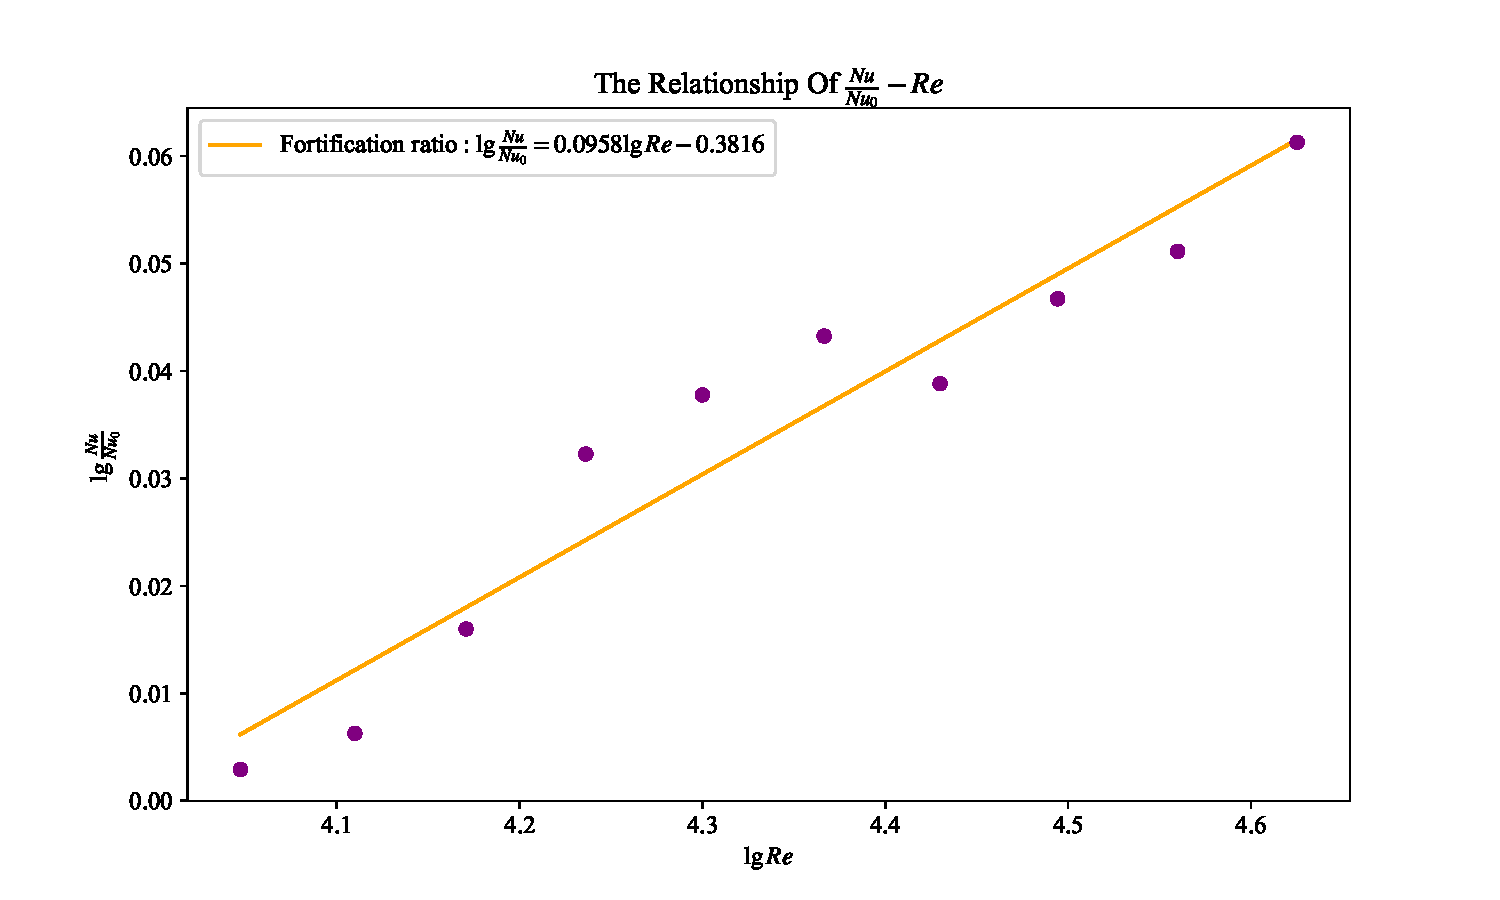
\includegraphics[scale=0.5]{强化比}
	\caption{$\frac{Nu}{Nu_{0}}$(强化比)与$Re$之关系(双对数坐标)}
	\label{fi3}
\end{figure}
\newpage

\begin{figure}[h]
	\centering
	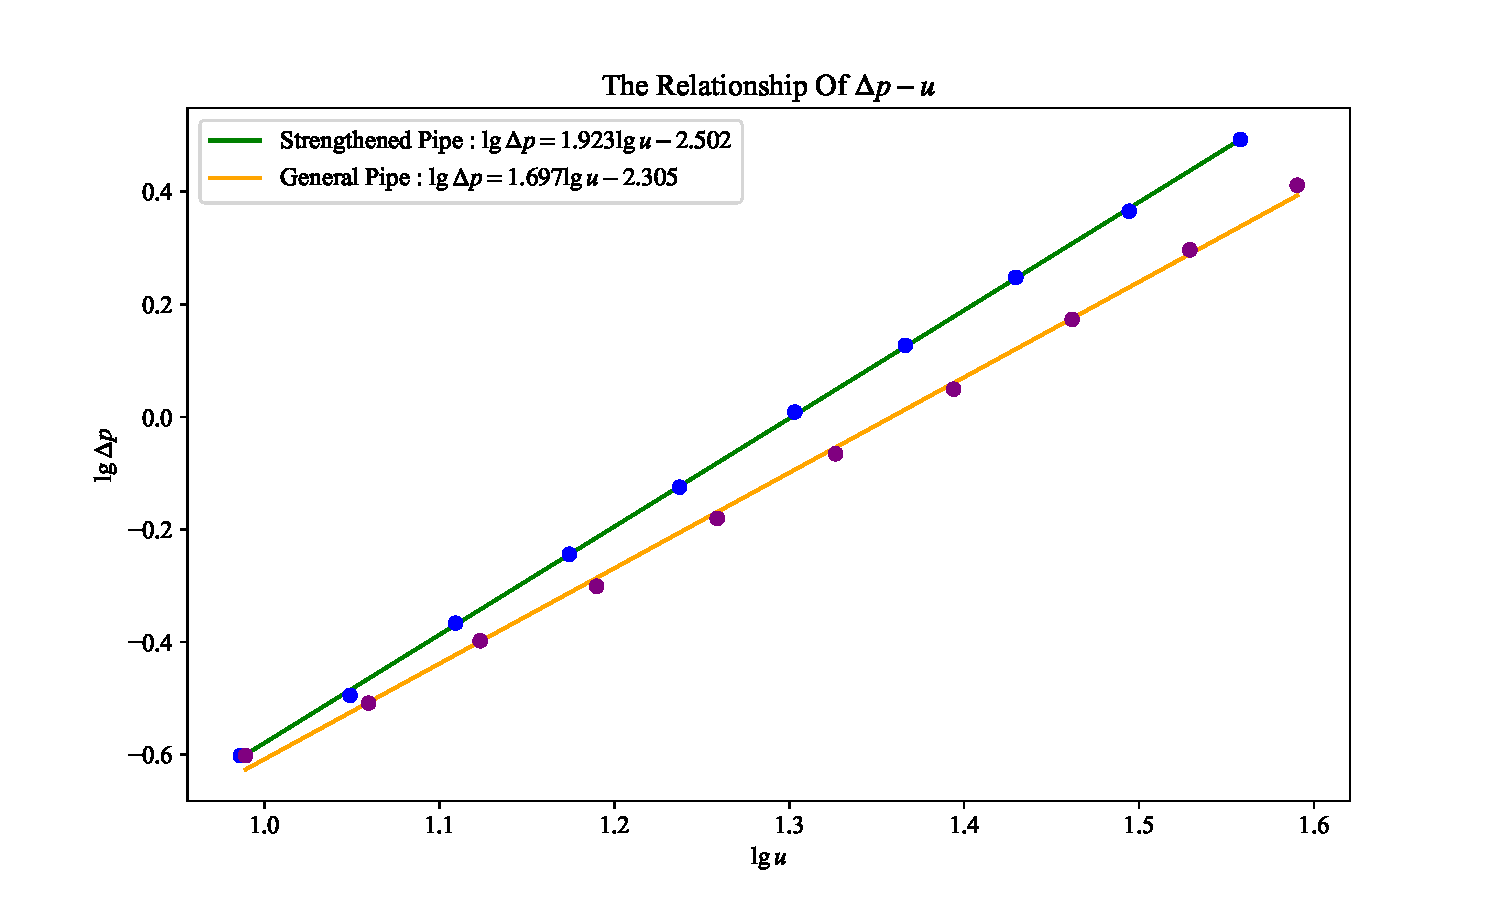
\includegraphics[scale=0.5]{压降}
	\caption{强化管、普通管的$\Delta p $(压降,去单位为kPa)与$u$(流速,去单位为m/s)之关系(双对数坐标)}
	\label{fi3}
\end{figure}


\newpage
\section{精馏综合实验}
\newpage
\begin{figure}[h]
	\centering
	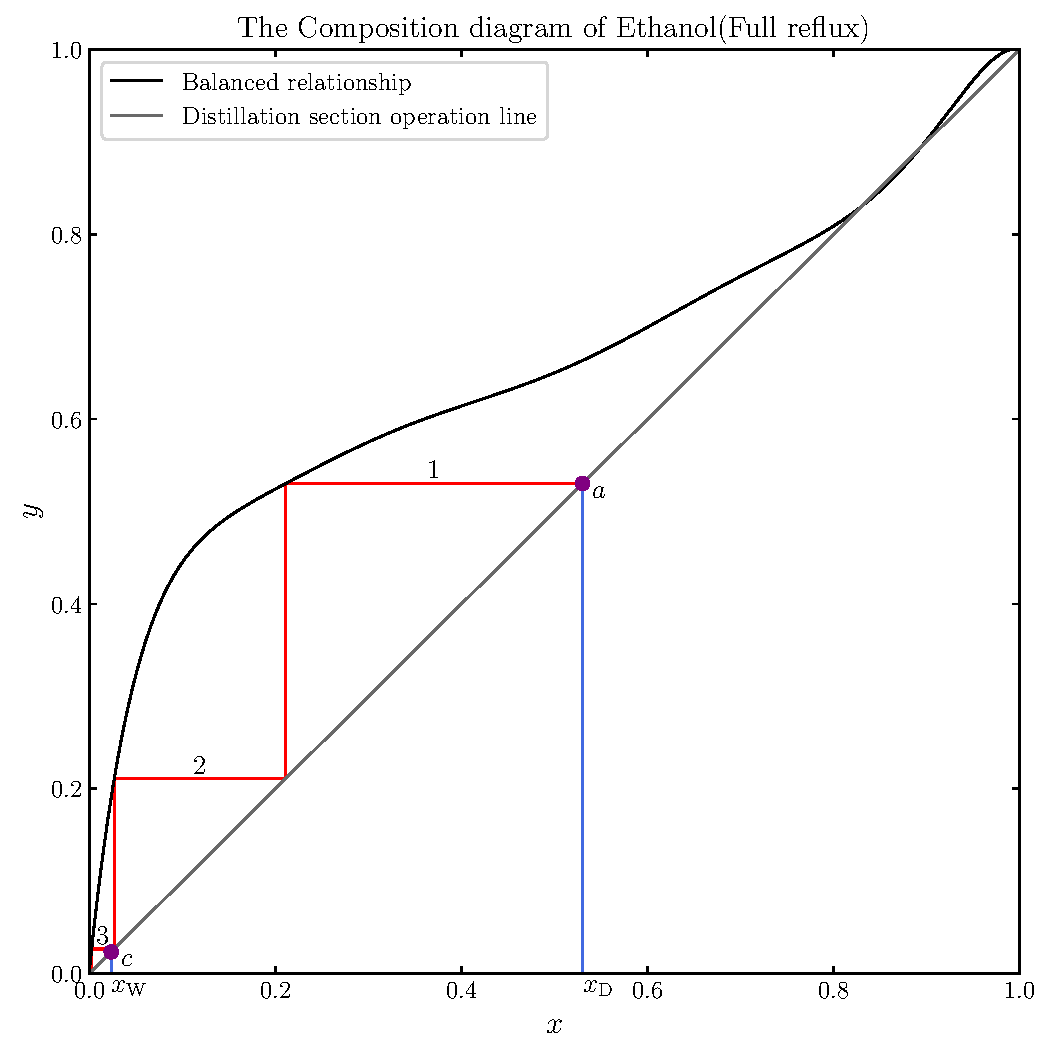
\includegraphics[scale=0.6]{全回流}
	\caption{二组分常压连续精馏-全回流-理论塔板数计算,计算结果为理论板数(取整)$N_{\rm{T}} = 3$。}
	\label{fi3}
\vspace*{20pt}
	\centering
	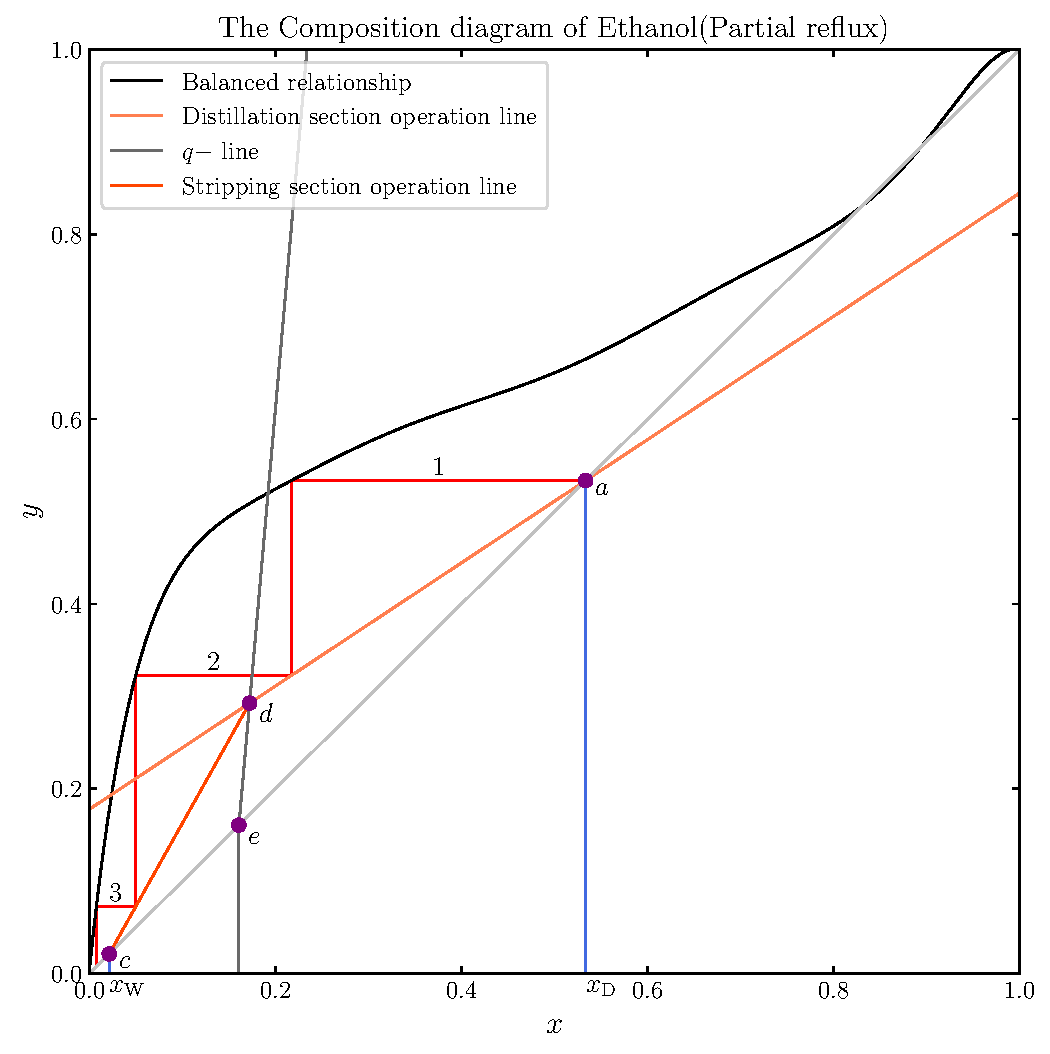
\includegraphics[scale=0.6]{部分回流}
	\caption{二组分常压连续精馏-部分回流-理论塔板数计算,计算结果为理论板数(取整)$N_{\rm{T}} = 3$。}
	\label{fi3}
\end{figure}

\newpage
\section{填料吸收综合实验}
\setcounter{figure}{4}
\begin{figure}[h]
	\centering
	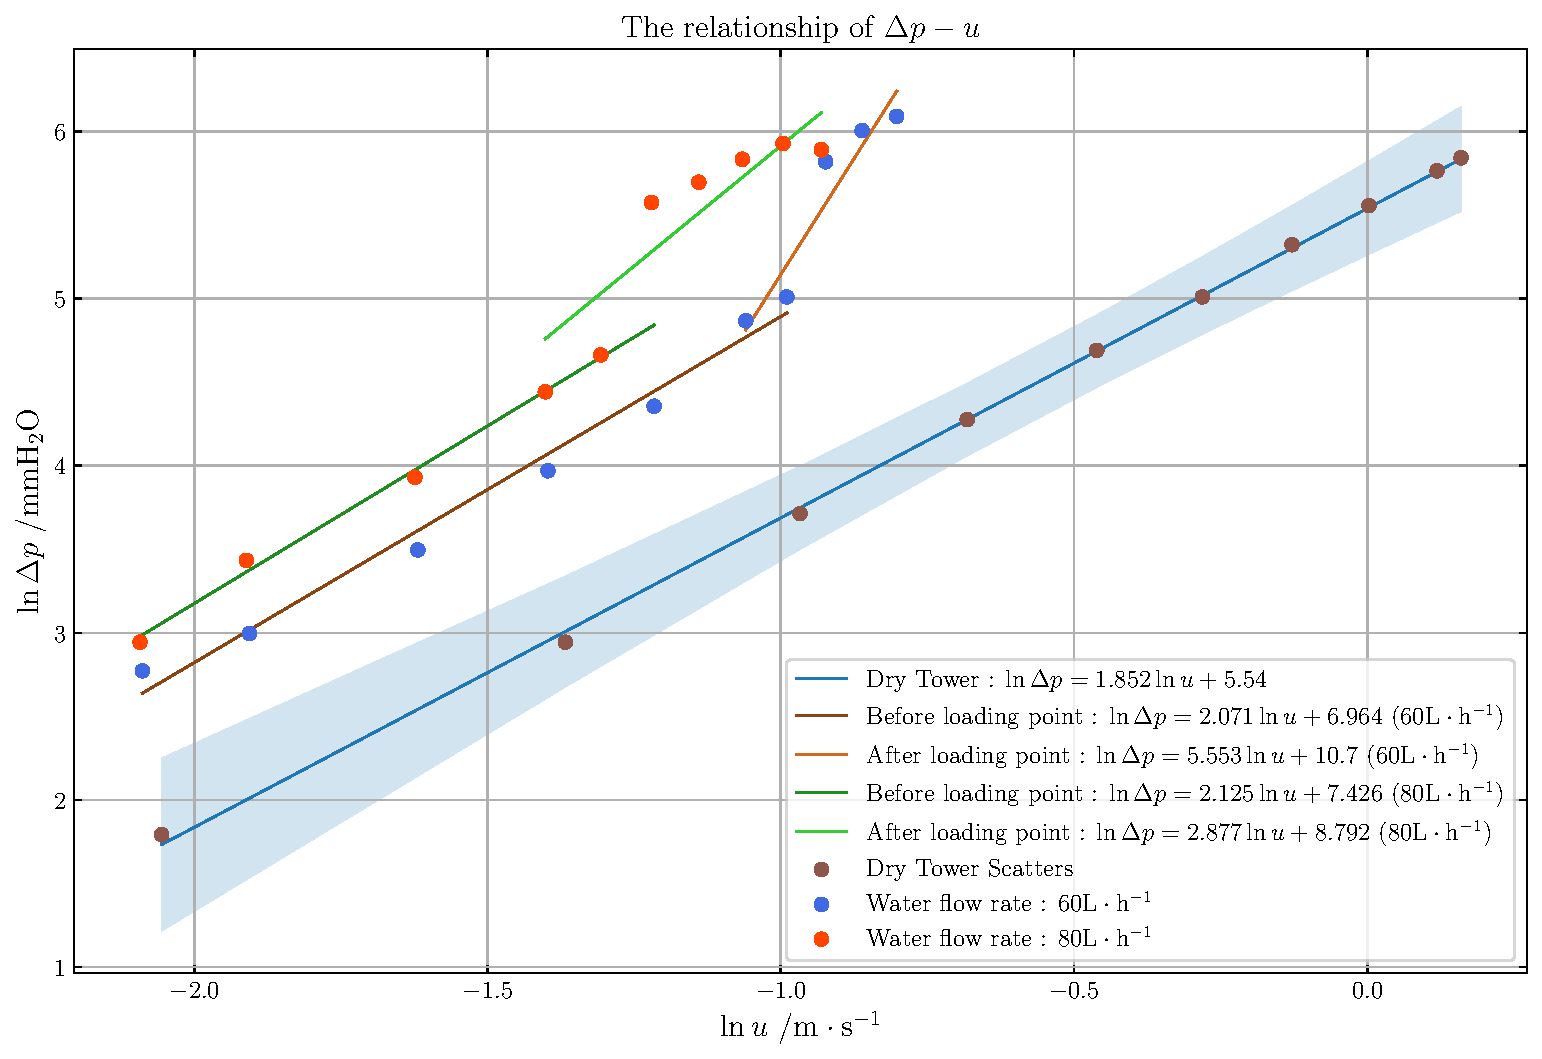
\includegraphics[scale=0.6]{填料吸收}
	\caption{干塔填料层压降$\Delta p$与空塔气速$u$之关系、L = 60$\rm{L}\cdot\rm{h}^{-1}$时的关系曲线、L = 80$\rm{L}\cdot\rm{h}^{-1}$时的关系曲线;横坐标为填料层压降$\Delta p$(去单位为$\rm{mmH}_{2}\rm{O}$,纵坐标为空塔气速$u$(去单位为$\rm{m}\cdot\rm{s}^{-1}$)}
	\vspace*{20pt}
	\centering
	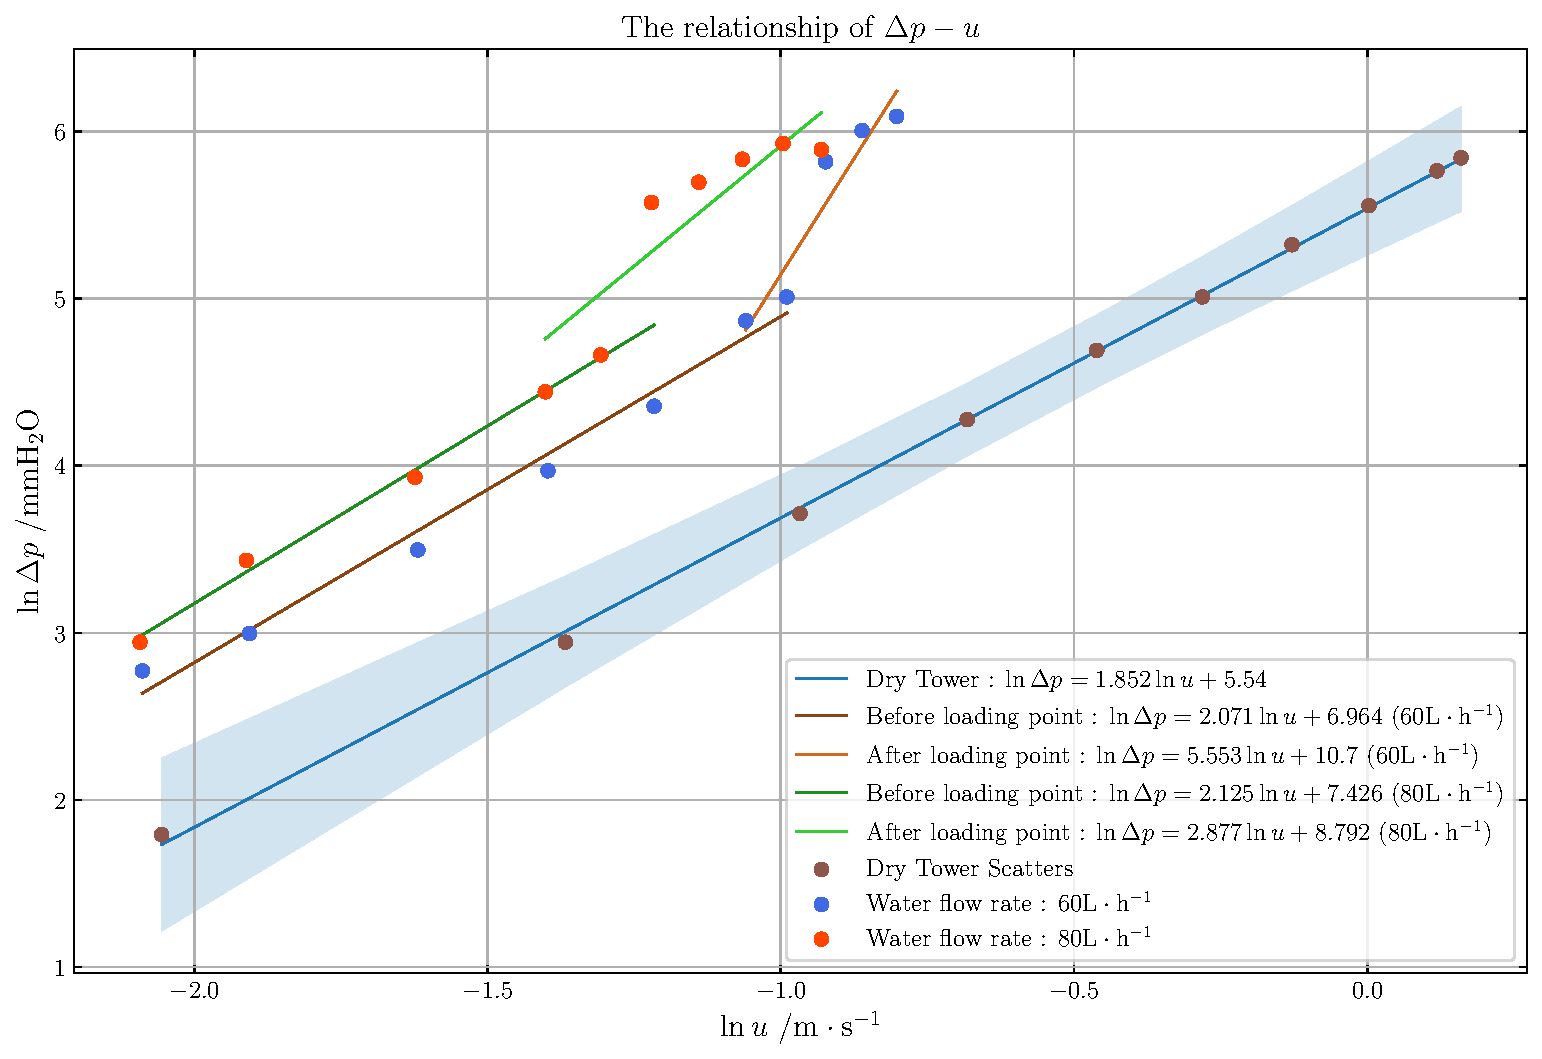
\includegraphics[scale=0.5]{填料吸收}
	\caption{干塔填料层压降$\Delta p$与空塔气速$u$之关系、L = 60$\rm{L}\cdot\rm{h}^{-1}$时的关系曲线、L = 80$\rm{L}\cdot\rm{h}^{-1}$时的关系曲线;横坐标为填料层压降$\Delta p$(去单位为$\rm{mmH}_{2}\rm{O}$,纵坐标为空塔气速$u$(去单位为$\rm{m}\cdot\rm{s}^{-1}$)}
\end{figure}
\setcounter{table}{0}

\setcounter{table}{0}
\begin{table}[h]
\caption{干塔数据及处理}
		\centering
		\begin{tabular}{p{3cm}<{\centering} p{3cm}<{\centering} p{3cm}<{\centering} p{3cm}<{\centering} p{3cm}<{\centering} p{3cm}<{\centering}}
		\toprule
		
   序号 & 空气流量计读数 & 填料层压降 & 空气温度 & $V_{\rm{OB}}$ & $u$ \\ 

  量纲&$\rm{m}^{3}\cdot\rm{h}^{-1}$&$\rm{mm}\ce{H2O}$&$^\circ$C&$\rm{m}^{3}\cdot\rm{s}^{-1}$&$\rm{m}\cdot\rm{s}^{-1}$\\
 \midrule
             1 & 2.5 & 6 & 23.5 & 0.0006433 & 0.1280 \\ 
        2 & 5.0 & 19 & 26.2 & 0.001281 & 0.2548 \\ 
        3 & 7.5 & 41 & 29.5 & 0.001911 & 0.3801 \\ 
        4 & 10.0 & 72 & 31.0 & 0.002541 & 0.5056 \\ 
        5 & 12.5 & 109 & 32.4 & 0.003169 & 0.6305 \\ 
        6 & 15.0 & 150 & 33.8 & 0.003794 & 0.7549 \\ 
        7 & 17.5 & 205 & 34.6 & 0.004421 & 0.8795 \\ 
        8 & 20.0 & 259 & 36.0 & 0.005041 & 1.003 \\ 
        9 & 22.5 & 319 & 37.0 & 0.005662 & 1.126 \\ 
        10 & 23.5 & 345 & 38.6 & 0.005899 & 1.173 \\ 		
        \bottomrule
		\end{tabular}	
		\label{ta1}
		
\end{table}


\begin{table}[h]
\caption{湿塔数据及处理$(L = 60 \rm{L}\cdot\rm{h}^{-1})$}
		\centering
		\begin{tabular}{p{1.5cm}<{\centering} p{3cm}<{\centering} p{3cm}<{\centering} p{2cm}<{\centering} p{2cm}<{\centering} p{3cm}<{\centering} p{3cm}<{\centering}}
		\toprule
		
   序号 & 空气流量计读数 & 填料层压降 & 空气温度&水温 & $V_{\rm{OB}}$ & $u$ \\ 

  量纲&$\rm{m}^{3}\cdot\rm{h}^{-1}$&$\rm{mm}\ce{H2O}$&$^\circ$C&$^\circ$C&$\rm{m}^{3}\cdot\rm{s}^{-1}$&$\rm{m}\cdot\rm{s}^{-1}$\\
 \midrule
             1 & 2.5 & 16 & 43.6 & 13.3 & 0.0006225 & 0.1239 \\ 
        2 & 3.0 & 20 & 43.4 & 13.3 & 0.0007473 & 0.1487 \\ 
        3 & 4.0 & 33 & 43.8 & 13.4 & 0.0009957 & 0.1981 \\ 
        4 & 5.0 & 53 & 44.6 & 13.4 & 0.001243 & 0.2473 \\ 
        5 & 6.0 & 78 & 45.4 & 13.4 & 0.001490 & 0.2964 \\ 
        6 & 7.0 & 130 & 44.0 & 13.3 & 0.001742 & 0.3466 \\ 
        7 & 7.5 & 150 & 43.4 & 13.3 & 0.001868 & 0.3717 \\ 
        8 & 8.0 & 337 & 42.4 & 13.6 & 0.001996 & 0.3971 \\ 
        9 & 8.5 & 406 & 41.4 & 13.7 & 0.002124 & 0.4226 \\ 
        10 & 9.0 & 442 & 40.2 & 14.4 & 0.002253 & 0.4483 \\ 		
        \bottomrule
		\end{tabular}	
		\label{ta1}
		
\end{table}
\newpage

\begin{table}[h]
\caption{湿塔数据及处理$(L = 80 \rm{L}\cdot\rm{h}^{-1})$}
		\centering
		\begin{tabular}{p{1.5cm}<{\centering} p{3cm}<{\centering} p{3cm}<{\centering} p{2cm}<{\centering} p{2cm}<{\centering} p{3cm}<{\centering} p{3cm}<{\centering}}
		\toprule
		
   序号 & 空气流量计读数 & 填料层压降 & 空气温度&水温 & $V_{\rm{OB}}$ & $u$ \\ 

  量纲&$\rm{m}^{3}\cdot\rm{h}^{-1}$&$\rm{mm}\ce{H2O}$&$^\circ$C&$^\circ$C&$\rm{m}^{3}\cdot\rm{s}^{-1}$&$\rm{m}\cdot\rm{s}^{-1}$\\
 \midrule
            1 & 2.5 & 19 & 46.2 & 13.3 & 0.0006200 & 0.1233 \\ 
        2 & 3.0 & 31 & 46.8 & 13.3 & 0.000743303 & 0.1479 \\ 
        3 & 4.0 & 51 & 47.0 & 13.4 & 0.0009908 & 0.1971 \\ 
        4 & 5.0 & 85 & 47.5 & 13.4 & 0.001237 & 0.2462 \\ 
        5 & 5.5 & 106 & 47.9 & 13.3 & 0.001360 & 0.2706 \\ 
        6 & 6.0 & 264 & 48.1 & 13.4 & 0.001484 & 0.2952 \\ 
        7 & 6.5 & 298 & 47.9 & 13.4 & 0.001608 & 0.3198 \\ 
        8 & 7.0 & 342 & 47.8 & 13.4 & 0.001732 & 0.3445 \\ 
        9 & 7.5 & 376 & 47.5 & 13.2 & 0.001856 & 0.3693 \\ 
        10 & 8.0 & 362 & 47.0 & 13.2 & 0.001982 & 0.3942 \\ 		
        \bottomrule
		\end{tabular}	
		\label{ta1}
		
\end{table}



\begin{table}[h]
\caption{填料吸收塔传质实验数据现象记录}
		\centering
		\begin{tabular}{p{2cm}<{\centering} p{10cm}<{\centering} p{4cm}<{\centering}}
		\toprule
		
      序号 & 名称 & 记录 \\ 

 \midrule
    
        1 & 填料种类 & 拉西环 \\ 
        2 & 填料层高度$h $ & 1m \\ 
        3 & \ce{CO2}转子流量计读数$V_{\ce{CO2}}$ & $0.3\rm{m}^{3}\cdot\rm{h}^{-1}$ \\ 
        4 & \ce{CO2}转子流量计处温度$T_{\ce{CO2}}$ &$35.6^{\circ}$C \\ 
        5 & 空气转子流量计读数$V_{\text{空气}}$ & $0.7\rm{m}^{3}\cdot\rm{h}^{-1}$ \\ 
        6 & 水转子流量计读数$V_{sL}$& $80\rm{L}\cdot\rm{h}^{-1}$ \\ 
        7 & 中和\ce{CO2}用\ce{Ba(OH)2}的浓度$c_{\ce{Ba(OH)2}}$ & $0.1013\rm{mol}\cdot\rm{L}^{-1}$ \\ 
        8 & 中和\ce{CO2}用\ce{Ba(OH)2}的体积$V_{\ce{Ba(OH)2}}$  & $10.00\rm{mL}$ \\ 
        9 & 滴定用盐酸的浓度$c_{\ce{HCl}}$ & $0.1106\rm{mol}\cdot\rm{L}^{-1}$ \\ 
        10 & 滴定塔底吸收液消耗盐酸的体积$V_{\text{底}\ce{HCl}}$ & $14.56\rm{mL}$ \\ 
        11 & 滴定用样品的体积$V_{\text{溶液}}$ & $20.00\rm{mL}$ \\ 
        12 & 塔底液相的温度$T_{\text{液}}$ & $13.1^{\circ}$C\\ 
        \bottomrule
		\end{tabular}	
		\label{ta1}
		
\end{table}




\end{document}
